\documentclass[12pt,a4paper]{article}
\usepackage[utf8]{inputenc}
\usepackage[russian]{babel}
\usepackage[OT1]{fontenc}
\usepackage{graphicx}
\usepackage{calc}
\usepackage[margin=15mm]{geometry}
% счётчик задач
\newcounter{notask}
\setcounter{notask}{1}

% условие без картинки
\newcommand{\task}[2]{
\hrule
\hbox to \textwidth {%
     \vrule
\parbox[t]{0.04\textwidth}{\smallskip \centering #1}%
     \vrule%
\hfill%
     \parbox[t]{0.93\textwidth}{\smallskip #2 \smallskip}\hfill%
\vrule
}
\hrule
    \addtocounter{notask}{1}
    \pagebreak[2]
}

\newlength{\h}
\newsavebox{\taskbox}
\newlength{\x}
\newsavebox{\pictbox}

% условие с картинкой (картинка выравнивается по центру)
\newcommand{\taskpic}[3]{
\savebox{\taskbox}{\parbox[t]{0.93\textwidth-4.3cm}{\smallskip #2 \smallskip}}
\savebox{\pictbox}{\parbox[t]{4cm}{\smallskip \centering
     \vspace{0pt} #3 \smallskip}}
\h=\ht\taskbox
\advance\h\dp\taskbox
\x=\ht\pictbox
\advance\x\dp\pictbox
\hrule
\hbox to \textwidth {%
\vrule\parbox[t][\maxof{\h}{\x}][t]{0.04\textwidth}{ \smallskip
     \centering #1 }\vrule%
\hfill\parbox[t][\maxof{\h}{\x}][t]{0.93\textwidth-4.3cm}{\smallskip #2
     \smallskip}\hfill\vrule%
\hfill\parbox[t][\maxof{\h}{\x}][c]{4cm}{\hfil #3 \hfil}\hfill\vrule
}
\hrule
\addtocounter{notask}{1}
\pagebreak[2]
}
\pagestyle{empty}


\begin{document}
\begin{center}
\begin{Large}
\textsc{ГЦФО. 9 класс. 2014/15.}
\end{Large}
\end{center}

\taskpic{3}{На расстоянии $L=2$~м от кошки сидели мышка и лягушка. Кошка прыгнула так, чтобы поймать их за раз, в этот момент мышь начала убегать, двигаясь по прямой с постоянной скоростью, а лягушка подпрыгнула вертикально с начальной скоростью $U=4$~м/с (см. рис.). Кошка поймала лягушку на лету, а мышку --- при приземлении. Известно, что мышь была поймана через 0{,}8~с после старта. Модуль начальной скорости кошки равен 5~м/с. Найдите скорость мышки и синус угла, под которым прыгнула кошка. Ускорение свободного падения считать равным $g=10$~м/с$^2$. Всех животных считать материальными точками, которые двигаются в одной плоскости. Сопротивлением воздуха пренебречь, пойманная лягушка не влияет на траекторию кошки.}{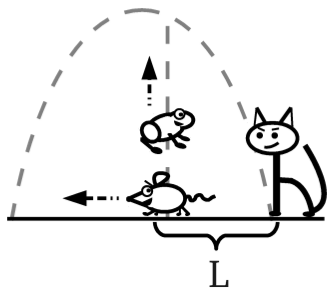
\includegraphics[width=4cm]{3}}

\end{document}